% ============================================================
% M2 轮4 S3 · 练习件 第4课时（§1.1.3 课1 空间直角坐标系与空间向量的坐标）
% 题面：照题面库 成卷/题面库/课时04-1.1.3课1.md 全 16 题冻结入卷（卷面题号＝库序 1~16）；
%       组名/难度照库头第 3/4 字段（第7/12题组名标「题组/解答」但题面带选项→照题面单选形制，登记）。
%       第14题设问后补排除说明「（论断②不作条件，不作结论．）」（定稿B §8.2 改字不改果，落台账）。
% 模板基线＝练习线样张（六宏零改动拷入）；版式＝练习线 p2 课时训练
%       （\keshi＋multicols＋花形三档 基础巩固1~10／综合提升11~14／思维探索15~16）。
% 图源：第9题＝单元4 image2+image3 双图行（各38mm）；第10题＝单元4 image8.png(30mm)；
%       第11题＝讲上 image9.png→js_image9.png(30mm，改名避让第12题)；第12题＝单元4 image9.png(27mm)；
%       第14题＝单元6 image24.png(30mm)。
% 取值/组名照登对照/图位/登记事项：见 ../批1值台账.md 课时04 节。
% 编译：xelatex main.tex（两遍）→ python render.py → png/pageN.png
% ============================================================
\documentclass[fontset=none]{ctexart}
\usepackage{qp-m3} % 换装：六宏→qp-m3 单包（钉后版 md5 7c3930362be8a0a2bdf21bbf8ac16573，两补钉随版）

% ============================================================
% 练习件局部宏（照练习线样张页2形制搬入；本段只加件，不改件）
% ============================================================
\renewcommand{\qpjianming}{练习件}
\renewcommand{\qpceming}{高中数学\quad 选择性必修第一册(人教B版)} % 换装回钉：qp-m3 默认册名＝选必二，防页脚漂移（试迁规约·试迁报告§四 B3 实证必改）
\renewcommand{\qpzhangming}{第一章\quad 空间向量与立体几何}

% ---------- YJ-01 灰块页脚·练习册档（块 31.0×7.8mm，照练习线样张 31.0mm 修正版） ----------
\newcommand{\qpxsyema}{\ifnum\value{page}<10 00\fi\ifnum\value{page}>9 \ifnum\value{page}<100 0\fi\fi\arabic{page}}
\newcommand{\lxshuziL}{\hbox to 13.8mm{\setlength{\fboxsep}{0pt}\colorbox{pnumbg}{%
  \makebox[31.0mm][l]{\rule[-3.145mm]{0pt}{7.8mm}\hspace{2.8mm}\fontsize{10.7pt}{13pt}\selectfont\color{black}\numpnum\qpxsyema}}\hss}}
\newcommand{\lxshuziR}{\hbox to 13.8mm{\kern-17.2mm\setlength{\fboxsep}{0pt}\colorbox{pnumbg}{%
  \makebox[31.0mm][r]{\rule[-3.145mm]{0pt}{7.8mm}\fontsize{10.7pt}{13pt}\selectfont\color{black}\numpnum\qpxsyema\hspace{2.75mm}}}}}
\fancyfoot[RO]{\raisebox{-1.24mm}[0pt][0pt]{\qphuitext\qpzhangming\quad{\heiti\qpjianming}\hspace{3mm}\lxshuziL}}
\fancyfoot[LE]{\raisebox{-1.24mm}[0pt][0pt]{\lxshuziR\hspace{3mm}\qphuitext\qpceming}}

% ---------- HX-01 花形·三档名（练习册版 25.5×6.8mm，重叠 o＝5.1mm） ----------
% 局部宏 \huadianOverlapLx 已由 qp-m3 收编（等值定义），依换装方案§1.4 预删防撞名
% 局部宏 \dangbadge 已由 qp-m3 收编（等值定义），依换装方案§1.4 预删防撞名

% ---------- TJ-02 练习册悬挂题号（单号 5.75mm／双位 7.6mm） ----------
% 长度 \lxhang 已由 qp-m3 分配，预删防重复定义
% 局部宏 \tihao 已由 qp-m3 收编（等值定义），依换装方案§1.4 预删防撞名
% 局部宏 \lxopt 已由 qp-m3 收编（等值定义），依换装方案§1.4 预删防撞名
% 局部宏 \xiexwei 已由 qp-m3 收编（等值定义），依换装方案§1.4 预删防撞名
% 局部宏 \zu 已由 qp-m3 收编（等值定义），依换装方案§1.4 预删防撞名

\begin{document}

% ============================================================
% 课时训练（三档 10＋4＋2＝16 题）
% ============================================================
\keshi{第4课时\quad 空间直角坐标系与空间向量的坐标}
\begin{multicols}{2}
\emergencystretch=1em

\dangbadge{基}{础}{巩}{固}

\tihao{1}\zu{cc1 正交基底与向量坐标×计算题组} \tieside{简单}已知\(\{\overrightarrow{e_1},\overrightarrow{e_2},\overrightarrow{e_3}\}\)是单位正交基底，分别写出下列空间向量的坐标：
\lxopt{(1)\(\overrightarrow{p}=-\overrightarrow{e_1}+\overrightarrow{e_2}-2\overrightarrow{e_3}\)；}
\lxopt{(2)\(\overrightarrow{q}=\overrightarrow{e_1}-\overrightarrow{e_2}\)；}
\lxopt{(3)\(\overrightarrow{r}=2\overrightarrow{e_2}+3\overrightarrow{e_3}\)．}
\xiexwei{16mm}
\begin{ansblock}[练-课时04-1]
% ans:练-课时04-1
\ansitem{1}{(1)\((-1,1,-2)\)；(2)\((1,-1,0)\)；(3)\((0,2,3)\)}
\end{ansblock}

\tihao{2}\zu{coordvec 两点求向量坐标×题组} \tieside{简单}根据下列条件，分别求向量\(\overrightarrow{AB}\)的坐标：
\lxopt{(1)\(A(2,-3,-1)\)，\(B(-6,5,3)\)；}
\lxopt{(2)\(A(-2,3,6)\)，\(B(-8,-6,4)\)．}
\xiexwei{16mm}
\begin{ansblock}[练-课时04-2]
% ans:练-课时04-2
\ansitem{2}{(1)\((-8,8,4)\)；(2)\((-6,-9,-2)\)}
\end{ansblock}

\tihao{3}\zu{eq 向量线性方程求 x×题组} \tieside{简单}分别求满足下列条件的向量\(\overrightarrow{x}\)：
\lxopt{(1)\(2(-1,5,1)+4\overrightarrow{x}=(2,14,-2)\)；}
\lxopt{(2)\((3,7,1)+2\overrightarrow{x}=(6,10,4)-\overrightarrow{x}\)．}
\xiexwei{16mm}
\begin{ansblock}[练-课时04-3]
% ans:练-课时04-3
\ansitem{3}{(1)\((1,1,-1)\)；(2)\((1,1,1)\)}
\end{ansblock}

\tihao{4}\zu{mid 中点坐标公式×填空} \tieside{简单}已知点\(A(1,5,3)\)，\(B(3,1,4)\)，求线段\(AB\)中点的坐标．
\xiexwei{16mm}
\begin{ansblock}[练-课时04-4]
% ans:练-课时04-4
\ansitem{4}{\(\left(2,3,\dfrac{7}{2}\right)\)}
\end{ansblock}

\tihao{5}\zu{dist ｜OM｜公式推导×填空} \tieside{简单}已知\(M(x,y,z)\)为空间直角坐标系中的一点，\(O\)为坐标原点，求\(\overrightarrow{OM}\)的长．
\xiexwei{16mm}
\begin{ansblock}[练-课时04-5]
% ans:练-课时04-5
\ansitem{5}{\(|OM|=\sqrt{x^{2}+y^{2}+z^{2}}\)}
\end{ansblock}

\tihao{6}\zu{op2 坐标线性运算＋数量积三小问×题组} \tieside{简单}已知\(\overrightarrow{a}=(3,2,-1)\)，\(\overrightarrow{b}=(5,-3,2)\)，求：
\lxopt{(1)\(\overrightarrow{a}+2\overrightarrow{b}\)；}
\lxopt{(2)\(\overrightarrow{a}\cdot\overrightarrow{b}\)；}
\lxopt{(3)\((2\overrightarrow{a}+\overrightarrow{b})\cdot(\overrightarrow{a}-3\overrightarrow{b})\)．}
\xiexwei{16mm}
\begin{ansblock}[练-课时04-6]
% ans:练-课时04-6
\ansitem{6}{(1)\((13,-4,3)\)；(2)\(7\)；(3)\(-121\)}
\end{ansblock}

\tihao{7}\zu{sym1 坐标面/轴对称点＋向量坐标×题组} \tieside{简单}已知\(A(1,2,-1)\)关于面\(xOy\)的对称点为\(B\)，而\(B\)关于\(x\)轴的对称点为\(C\)，则\nobreak\(\overrightarrow{BC}\)等于\nobreak(\kongwei)
\lxopt{\makebox[\dimexpr0.5\linewidth-1em\relax][l]{A．\((0,4,2)\)；}\makebox[\dimexpr0.5\linewidth-1em\relax][l]{B．\((-2,0,0)\)}}
\lxopt{\makebox[\dimexpr0.5\linewidth-1em\relax][l]{C．\((0,-4,-2)\)；}\makebox[\dimexpr0.5\linewidth-1em\relax][l]{D．\((2,0,-2)\)}}
\begin{ansblock}[练-课时04-7]
% ans:练-课时04-7
\ansitem{7}{C（\((0,-4,-2)\)）}
\end{ansblock}

\tihao{8}\duoxuan\zu{sym2 对称点命题辨析×多选} \tieside{简单}在空间直角坐标系中，已知点\(P(x,y,z)\)，下列叙述正确的序号有\nobreak(\kongwei)
\lxopt{①点\(P\)关于\(x\)轴的对称点是\(P_1(x,-y,z)\)；}
\lxopt{②点\(P\)关于\(yOz\)平面的对称点是\(P_2(x,-y,-z)\)；}
\lxopt{③点\(P\)关于\(y\)轴的对称点是\(P_3(x,-y,z)\)；}
\lxopt{④点\(P\)关于原点的对称点是\(P_4(-x,-y,-z)\)}
\begin{ansblock}[练-课时04-8]
% ans:练-课时04-8
\ansitem{8}{④（仅④真）}
\end{ansblock}

\tihao{9}\zu{c2 长方体开放建系读全部顶点坐标×解答} \tieside{简单}如图，在长方体\(ABCD\text{-}\penalty100 A'B'C'D'\)中，\(AB=a\)，\(BC=b\)，\(CC'=c\)，将此长方体放在空间直角坐标系中的不同位置，分别说出长方体各个顶点的坐标．
\par\vspace{1.9mm}\penalty10000\noindent\makebox[\linewidth][c]{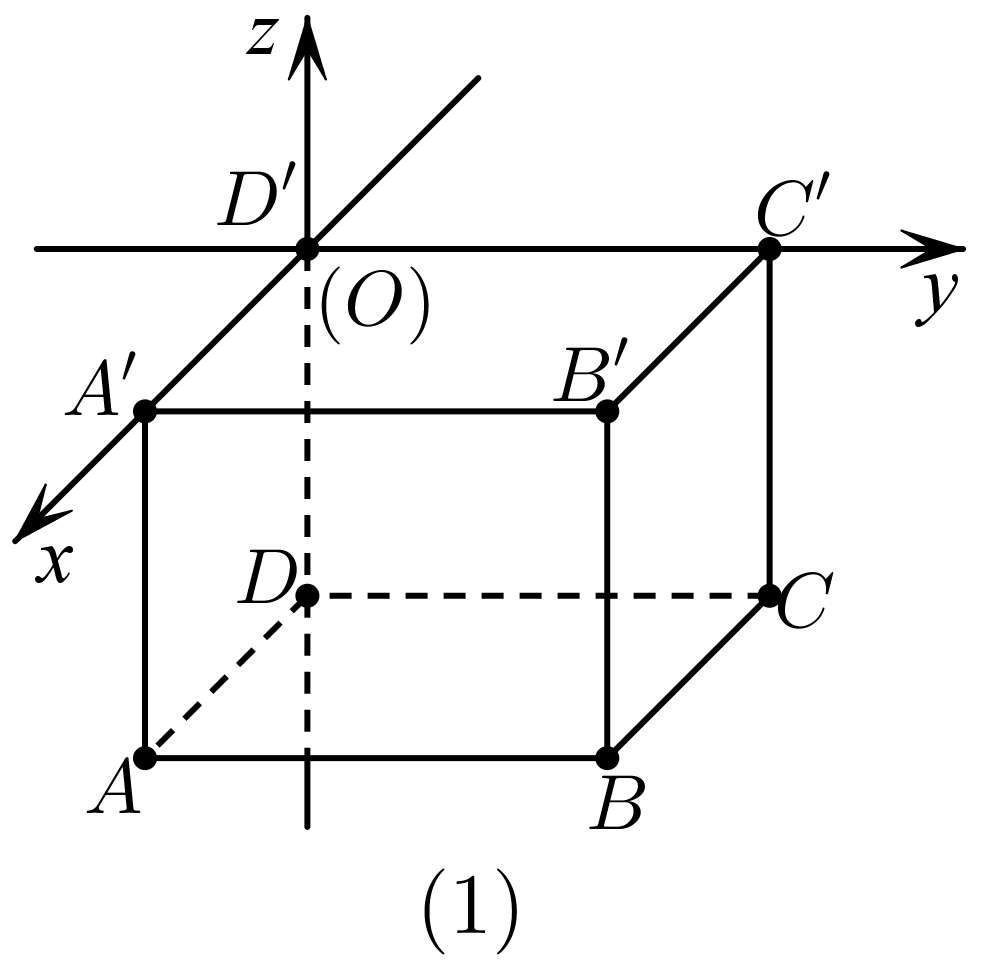
\includegraphics[width=38mm]{figs/dy4_image2.png}\hspace{4mm}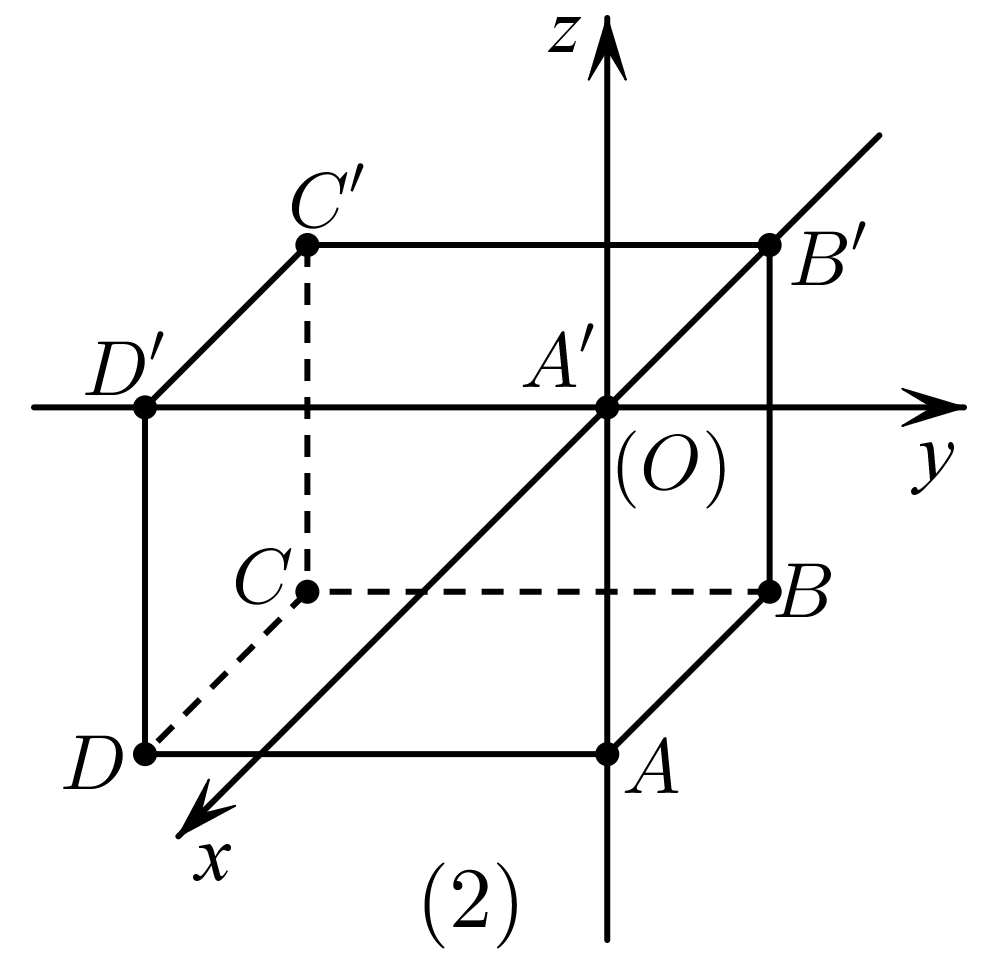
\includegraphics[width=38mm]{figs/dy4_image3.png}}\par\vspace{-1.0mm}\penalty-50
\xiexwei{16mm}
\begin{ansblock}[练-课时04-9]
% ans:练-课时04-9
\ansitem{9}{开放题（常见建系位逐顶点坐标）}
\end{ansblock}

\tihao{10}\zu{c3 按线段比写点坐标×单选} \tieside{简单}如图，正方体\(OABC\text{-}\penalty100 O_1A_1B_1C_1\)的棱长为\(2\)，\(E\)是\(B_1B\)上的点，且\(EB=2EB_1\)，则点\(E\)的坐标为\nobreak(\kongwei)
\par\vspace{1.9mm}\penalty10000\noindent\makebox[\linewidth][c]{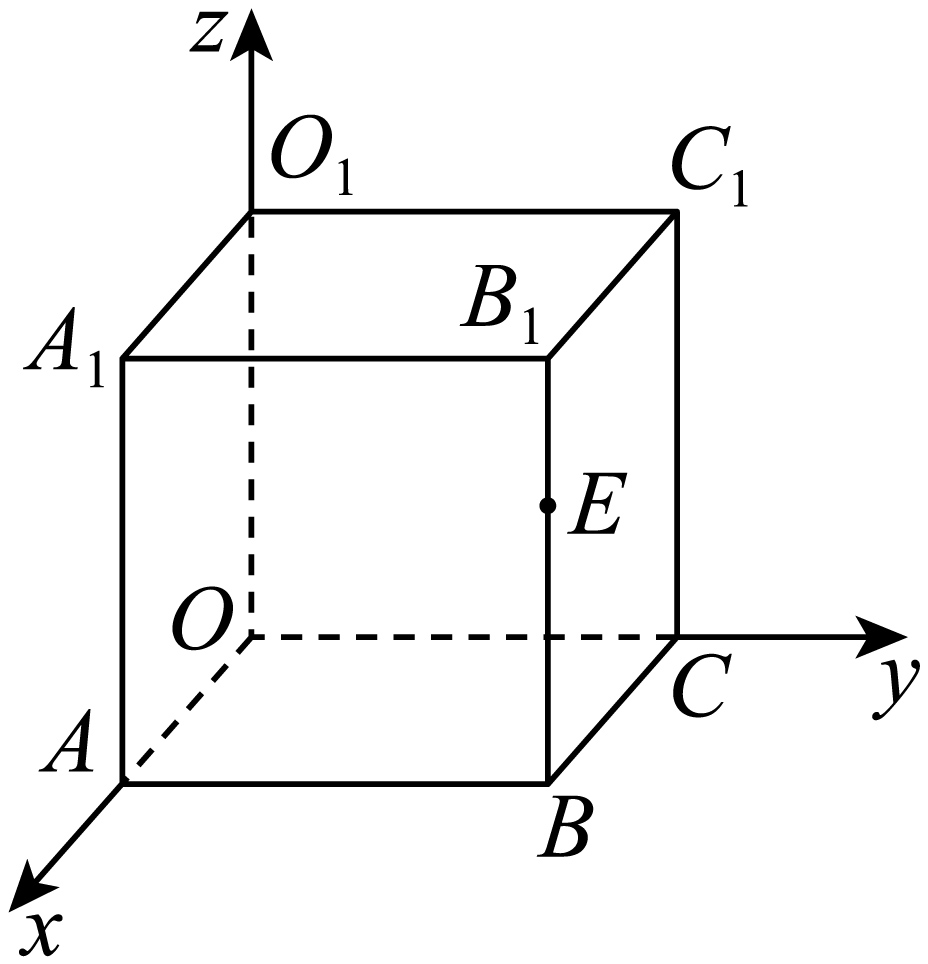
\includegraphics[width=30mm]{figs/dy4_image8.png}}\par\vspace{-1.0mm}\penalty10000
\lxopt{\makebox[\dimexpr0.25\linewidth-0.25\lxhang-0.25em\relax][l]{A．\((2,2,1)\)；}\makebox[\dimexpr0.25\linewidth-0.25\lxhang-0.25em\relax][l]{B．\((2,2,2)\)；}\makebox[\dimexpr0.25\linewidth-0.25\lxhang-0.25em\relax][l]{C．\((2,2,\frac{2}{3})\)；}\makebox[\dimexpr0.25\linewidth-0.25\lxhang-0.25em\relax][l]{D．\((2,2,\frac{4}{3})\)}}
\begin{ansblock}[练-课时04-10]
% ans:练-课时04-10
\setlength{\anshang}{7.6mm}% 题10 起双位档（照答案册同值，块内局部）
\ansitem{10}{D（\(\left(2,2,\dfrac{4}{3}\right)\)）}
\end{ansblock}

\dangbadge{综}{合}{提}{升}

\tihao{11}\zu{c1 建系写顶点／中点／动点坐标×三问递进} \tieside{中档}已知三棱锥\(P\text{-}\penalty100 ABC\)中，\(PA\perp\)平面\(ABC\)，\(AB\perp AC\)，若\(PA=3\)，\(AB=2\)，\(AC=2\)，建立空间直角坐标系．
\par\vspace{1.9mm}\penalty10000\noindent\makebox[\linewidth][c]{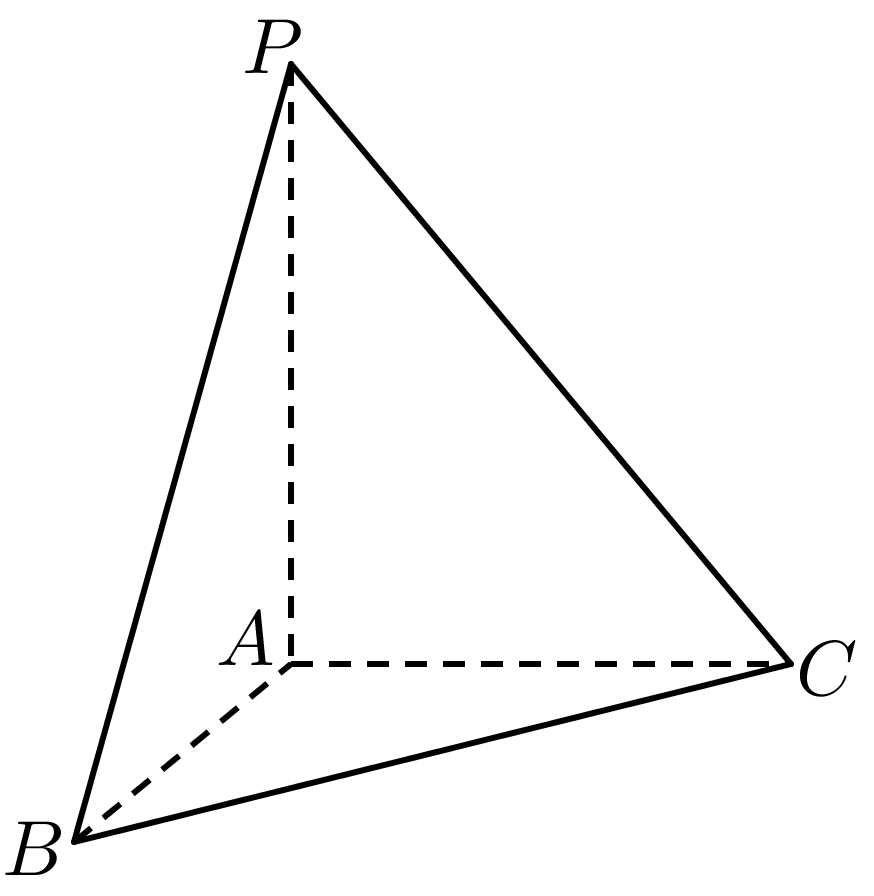
\includegraphics[width=30mm]{figs/js_image9.png}}\par\vspace{-1.0mm}\penalty10000
\lxopt{(1)求各顶点的坐标；}
\lxopt{(2)若点\(Q\)是\(PC\)的中点，求点\(Q\)坐标；}
\lxopt{(3)若点\(M\)在线段\(PC\)上移动，写出点\(M\)坐标．}
\xiexwei{16mm}
\begin{ansblock}[练-课时04-11]
% ans:练-课时04-11
\setlength{\anshang}{7.6mm}% 题11 起双位档（照答案册同值，块内局部）
\ansitem{11}{(1)\(A(0,0,0)\)，\(B(2,0,0)\)，\(C(0,2,0)\)，\(P(0,0,3)\)；(2)\(Q\left(0,1,\dfrac{3}{2}\right)\)；(3)\(M\left(0,t,3-\dfrac{3}{2}t\right)\)，\(t\in[0,2]\)}
\end{ansblock}

\tihao{12}\zu{c4 三面共轴正四面体求第四顶点坐标×解答} \tieside{中档}如图，棱长为\(\sqrt{2}\)的正四面体\(ABCD\)的三个顶点\(A\)，\(B\)，\(C\)分别在空间直角坐标系的坐标轴\(Ox\)，\(Oy\)，\(Oz\)上，\(D\)在第一卦限，则定点\(D\)的坐标为\nobreak(\kongwei)
\par\vspace{1.9mm}\penalty10000\noindent\makebox[\linewidth][c]{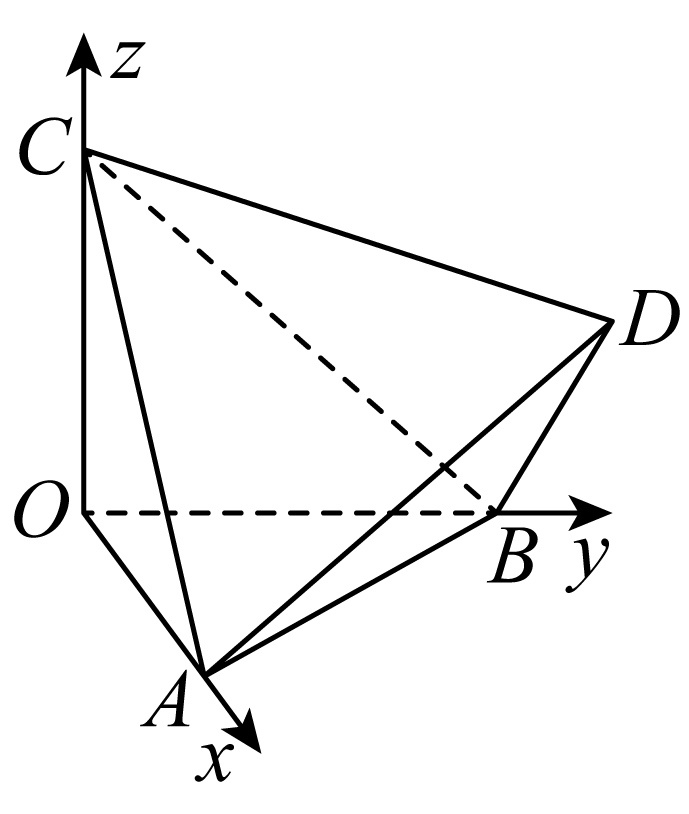
\includegraphics[width=27mm]{figs/dy4_image9.png}}\par\vspace{-1.0mm}\penalty10000
\lxopt{\makebox[\dimexpr0.5\linewidth-0.5\lxhang-0.25em\relax][l]{A．\((1,1,1)\)；}\makebox[\dimexpr0.5\linewidth-0.5\lxhang-0.25em\relax][l]{B．\((\sqrt{2},\sqrt{2},\sqrt{2})\)}}
\lxopt{\makebox[\dimexpr0.5\linewidth-0.5\lxhang-0.25em\relax][l]{C．\((\sqrt{3},\sqrt{3},\sqrt{3})\)；}\makebox[\dimexpr0.5\linewidth-0.5\lxhang-0.25em\relax][l]{D．\((2,2,2)\)}}
\begin{ansblock}[练-课时04-12]
% ans:练-课时04-12
\setlength{\anshang}{7.6mm}% 题12 起双位档（照答案册同值，块内局部）
\ansitem{12}{A（\((1,1,1)\)）}
\end{ansblock}

\tihao{13}\zu{c6 平行六面体顶点坐标（中心对称）×解答} \tieside{中档}已知空间直角坐标系中，平行六面体\(ABCD\text{-}\penalty100 A_1B_1C_1D_1\)满足：\(A(-2,1,3)\)，\(B(2,2,1)\)，\(C(3,4,2)\)，\(D(-1,3,4)\)，且平行六面体的体对角线的交点为\(M(1,1,1)\)，求\(A_1\)，\(B_1\)，\(C_1\)，\(D_1\)的坐标．
\xiexwei{16mm}
\begin{ansblock}[练-课时04-13]
% ans:练-课时04-13
\setlength{\anshang}{7.6mm}% 题13 起双位档（照答案册同值，块内局部）
\ansitem{13}{\(A_{1}(-1,-2,0)\)，\(B_{1}(3,-1,-2)\)，\(C_{1}(4,1,-1)\)，\(D_{1}(0,0,1)\)}
\end{ansblock}

\tihao{14}\zu{开放命题构造×垂直$\Leftrightarrow$面积等价（1.2.2 拓展认领入中槽）} \tieside{中档}如图，在棱长为\(2\)的正方体\(ABCD\text{-}\penalty100 A_1B_1C_1D_1\)中，点\(E\)为棱\(CD\)的中点，点\(F\)为底面\(ABCD\)内一点，给出下列三个论断：
\par\vspace{1.9mm}\penalty10000\noindent\makebox[\linewidth][c]{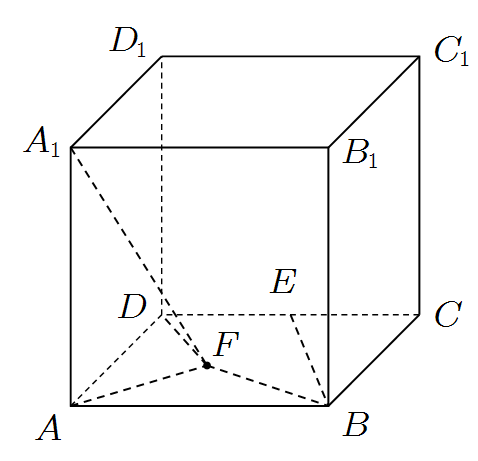
\includegraphics[width=30mm]{figs/dy6_image24.png}}\par\vspace{-1.0mm}\penalty10000
\lxopt{①\(A_1F\perp BE\)；}
\lxopt{②\(A_1F=3\)；}
\lxopt{③\(S_{\triangle ADF}=2S_{\triangle ABF}\)．}
\lxopt{以其中的一个论断作为条件，另一个论断作为结论，写出一个正确的命题：\kongbai{}（论断②不作条件，不作结论．）}
\begin{ansblock}[练-课时04-14]
% ans:练-课时04-14
\setlength{\anshang}{7.6mm}% 题14 起双位档（照答案册同值，块内局部）
\ansitem{14}{①\(\Leftrightarrow\)③（②不作条件，不作结论）}
\end{ansblock}

\dangbadge{思}{维}{探}{索}

\tihao{15}\zu{T10 轨迹范围型改造底·三问解答} \tieside{难}在棱长为\(4\)的正方体\(ABCD\text{-}\penalty100 A_1B_1C_1D_1\)中，点\(P\)在底面\(ABCD\)（含边界）内运动，且满足\(\overrightarrow{PA_1}\cdot\overrightarrow{PC_1}=m\)（\(m\)为常数）．
\lxopt{(1)以\(A\)为原点，\(\overrightarrow{AB}\)、\(\overrightarrow{AD}\)、\(\overrightarrow{AA_1}\)的方向为\(x\)轴、\(y\)轴、\(z\)轴正方向建立空间直角坐标系．当\(m=12\)时，求点\(P\)轨迹的方程，说明轨迹形状，并求轨迹的长度；}
\lxopt{(2)若点\(P\)的轨迹与底面正方形的边界恰好有\(4\)个公共点，求\(m\)的所有可能值；}
\lxopt{(3)当\(m=16\)时，求\(|\overrightarrow{PB_1}|\)的所有可能取值．}
\xiexwei{16mm}
\begin{ansblock}[练-课时04-15]
% ans:练-课时04-15
\setlength{\anshang}{7.6mm}% 题15 起双位档（照答案册同值，块内局部）
\ansitem{15}{(1)\((x-2)^{2}+(y-2)^{2}=4\)（\(m=12\)），圆，长 \(4\pi\)；(2)\(m=12\) 或 \(16\)；(3)\(|PB_{1}|\in\{4,\ 4\sqrt{2},\ 4\sqrt{3}\}\)}
\end{ansblock}

\tihao{16}\zu{T9 新定义型改造底·三问解答} \tieside{难}若三数轴\(Ox\)、\(Oy\)、\(Oz\)有公共原点\(O\)，且\(Ox\perp Oy\)，\(Oz\)与\(Ox\)、\(Oy\)的夹角均为\(60^\circ\)，则称其为「半直角斜坐标系」（这样的轴系确实存在：例如直角坐标系中取\(\overrightarrow{i}=(1,0,0)\)，\(\overrightarrow{j}=(0,1,0)\)，\(\overrightarrow{k}=(\frac{1}{2},\frac{1}{2},\frac{\sqrt{2}}{2})\)）．设\(\overrightarrow{i}\)、\(\overrightarrow{j}\)、\(\overrightarrow{k}\)分别为三轴正方向单位向量；若空间向量\(\overrightarrow{n}=x\overrightarrow{i}+y\overrightarrow{j}+z\overrightarrow{k}\)，则记\(\overrightarrow{n}=[x,y,z]\)，称为\(\overrightarrow{n}\)的（半直角）斜坐标．
\lxopt{(1)已知\(\overrightarrow{a}=[1,1,-2]\)，\(\overrightarrow{b}=[2,-1,1]\)，求\(\overrightarrow{a}\cdot\overrightarrow{b}\)；}
\lxopt{(2)求所有满足\(|\overrightarrow{v}|=2\)的实数\(t\)，其中\(\overrightarrow{v}=[t,t,2]\)；}
\lxopt{(3)对(2)中每个\(\overrightarrow{v}\)，分别求\(\overrightarrow{v}\)与\(\overrightarrow{w}=[1,1,0]\)夹角的余弦值，并指出夹角．}
\xiexwei{16mm}
\begin{ansblock}[练-课时04-16]
% ans:练-课时04-16
\setlength{\anshang}{7.6mm}% 题16 起双位档（照答案册同值，块内局部）
\ansitem{16}{(1)\(-1\)；(2)\(t=0\) 或 \(-2\)；(3)\(t=0\)：\(45^{\circ}\)；\(t=-2\)：\(135^{\circ}\)}
\end{ansblock}

\end{multicols}

\tailfill
\end{document}
